\section{Disjoint perfect matchings}

\begin{frame}{Disjoint perfect matchings as pages}

%Take disjoint perfect matchings as pages.
\newProb{\probMatching}
{Disjoint perfect matchings $E_1,\dotsc, E_k$ on a vertex
set $V$.}{Is there a book embedding of $(V, E_i)$?}

\begin{theorem}
Necessary: $G := (V, E_1 \cup \dotsb \cup E_k)$ is bipartite.
\end{theorem}

\begin{overprint}
\onslide<1>
\begin{itemize}
\item Even number of vertices between adjacent vertices in valid order
\begin{figure}
\centering

\resizebox{0.6\textwidth}{!}{
\begin{tikzpicture}
\node (v) {v};
\node[right of=v,node distance=7em] (nw) {$n_i(w)$};
\node[right of=nw,node distance=7em] (w) {$w$};
\node[right of=w,node distance=7em] (nv) {$n_i(v)$};

\draw (v) edge[bend left] (nv);
\draw (nw) edge[bend left] (w);

/* v to n1 */
\draw[decoration={brace},decorate,thick] ($ (nv) + (-1.2em, -1em) $) -- ($ (v) + (0.5em,-1em) $);
\node[text centered] at ($ 0.5*($(nv) + (v)$) + (-0.25em, -2em) $) {even};

\node[text centered] at ($ 0.5*($(v) + (nw)$) + (0.25em, 0)$) {\dots};
\node[text centered] at ($ 0.5*($(nw) + (w)$) + (0.25em, 0)$) {\dots};
\node[text centered] at ($ 0.5*($(w) + (nv)$) + (0.25em, 0)$) {\dots};
\end{tikzpicture}
}
\end{figure}
\end{itemize}

\onslide<2>
\begin{itemize}
\item Even number of vertices between adjacent vertices in valid order
\item[$\Rightarrow$] Vertices with even and odd indexes form bipartition
\end{itemize}
\end{overprint}

\end{frame}

\begin{frame}{Bipartite examples}
\begin{figure}[\placement]
\centering

\scalebox{1.3}{%
\begin{tikzpicture}

\node (l1) {{\relscale{0.5}$l_0$}};
\node[right of=l1,node distance=6em] (r1) {{\relscale{0.5}$r_0$}};
\node[below of=l1] (l2) {{\relscale{0.5}$l_1$}};
\node[right of=l2,node distance=6em] (r2) {{\relscale{0.5}$r_1$}};
\node[below of=l2] (l3) {{\relscale{0.5}$l_2$}};
\node[right of=l3,node distance=6em] (r3) {{\relscale{0.5}$r_2$}};
\node[below of=l3] (l4) {{\relscale{0.5}$l_3$}};
\node[right of=l4,node distance=6em] (r4) {{\relscale{0.5}$r_3$}};

\draw (l1) edge (r1);
\draw (l2) edge (r2);
\draw (l3) edge (r3);
\draw (l4) edge (r4);
\draw[edge1] (l1) edge (r2);
\draw[edge1] (l2) edge (r3);
\draw[edge1] (l3) edge (r4);
\draw[edge1] (l4) edge (r1);
\draw[edge2] (l1) edge (r3);
\draw[edge2] (l2) edge (r4);
\draw[edge2] (l3) edge (r1);
\draw[edge2] (l4) edge (r2);
\draw[edge3] (l1) edge (r4);
\draw[edge3] (l2) edge (r1);
\draw[edge3] (l3) edge (r2);
\draw[edge3] (l4) edge (r3);
\end{tikzpicture}}
\end{figure}

$k$ pages: Take the partition $E_i := \bigl\{\{l_j, r_{(j + i)\bmod{k}}\}: j \in \range{k-1}\bigr\}$ of $K_{k,k}$ 
\end{frame}

\begin{frame}{Bipartite counterexamples}
\begin{figure}[\placement]
\centering

\scalebox{1.3}{%
\begin{tikzpicture}

\node (l1) {{\relscale{0.5}$l_1$}};
\node[right of=l1,node distance=6em] (r1) {{\relscale{0.5}$r_1$}};
\node[below of=l1] (l2) {{\relscale{0.5}$l_2$}};
\node[right of=l2,node distance=6em] (r2) {{\relscale{0.5}$r_2$}};
\node[below of=l2] (l3) {{\relscale{0.5}$l_3$}};
\node[right of=l3,node distance=6em] (r3) {{\relscale{0.5}$r_3$}};
\node[below of=l3] (l4) {{\relscale{0.5}$l_4$}};
\node[right of=l4,node distance=6em] (r4) {{\relscale{0.5}$r_4$}};

\draw (l1) edge (r1);
\draw (l2) edge (r2);
\draw (l3) edge (r3);
\draw (l4) edge (r4);
\draw[edge1] (l1) edge (r2);
\draw[edge1] (l2) edge (r1);
\draw[edge1] (l3) edge (r4);
\draw[edge1] (l4) edge (r3);
\draw[edge2] (l1) edge (r3);
\draw[edge2] (l3) edge (r1);
\draw[edge2] (l2) edge (r4);
\draw[edge2] (l4) edge (r2);
\draw[edge3] (l1) edge (r4);
\draw[edge3] (l4) edge (r1);
\draw[edge3] (l2) edge (r3);
\draw[edge3] (l3) edge (r2);
\end{tikzpicture}}
\end{figure}

$k \geq 4$ pages: Partition $K_{k,k}$ into disjoint perfect matchings that contain
this counterexample
\end{frame}

\begin{frame}{Bipartite counterexample for three pages}
Smallest counterexample where two of the matchings form a cycle\vspace{-1em}
\begin{figure}[\placement]
\centering
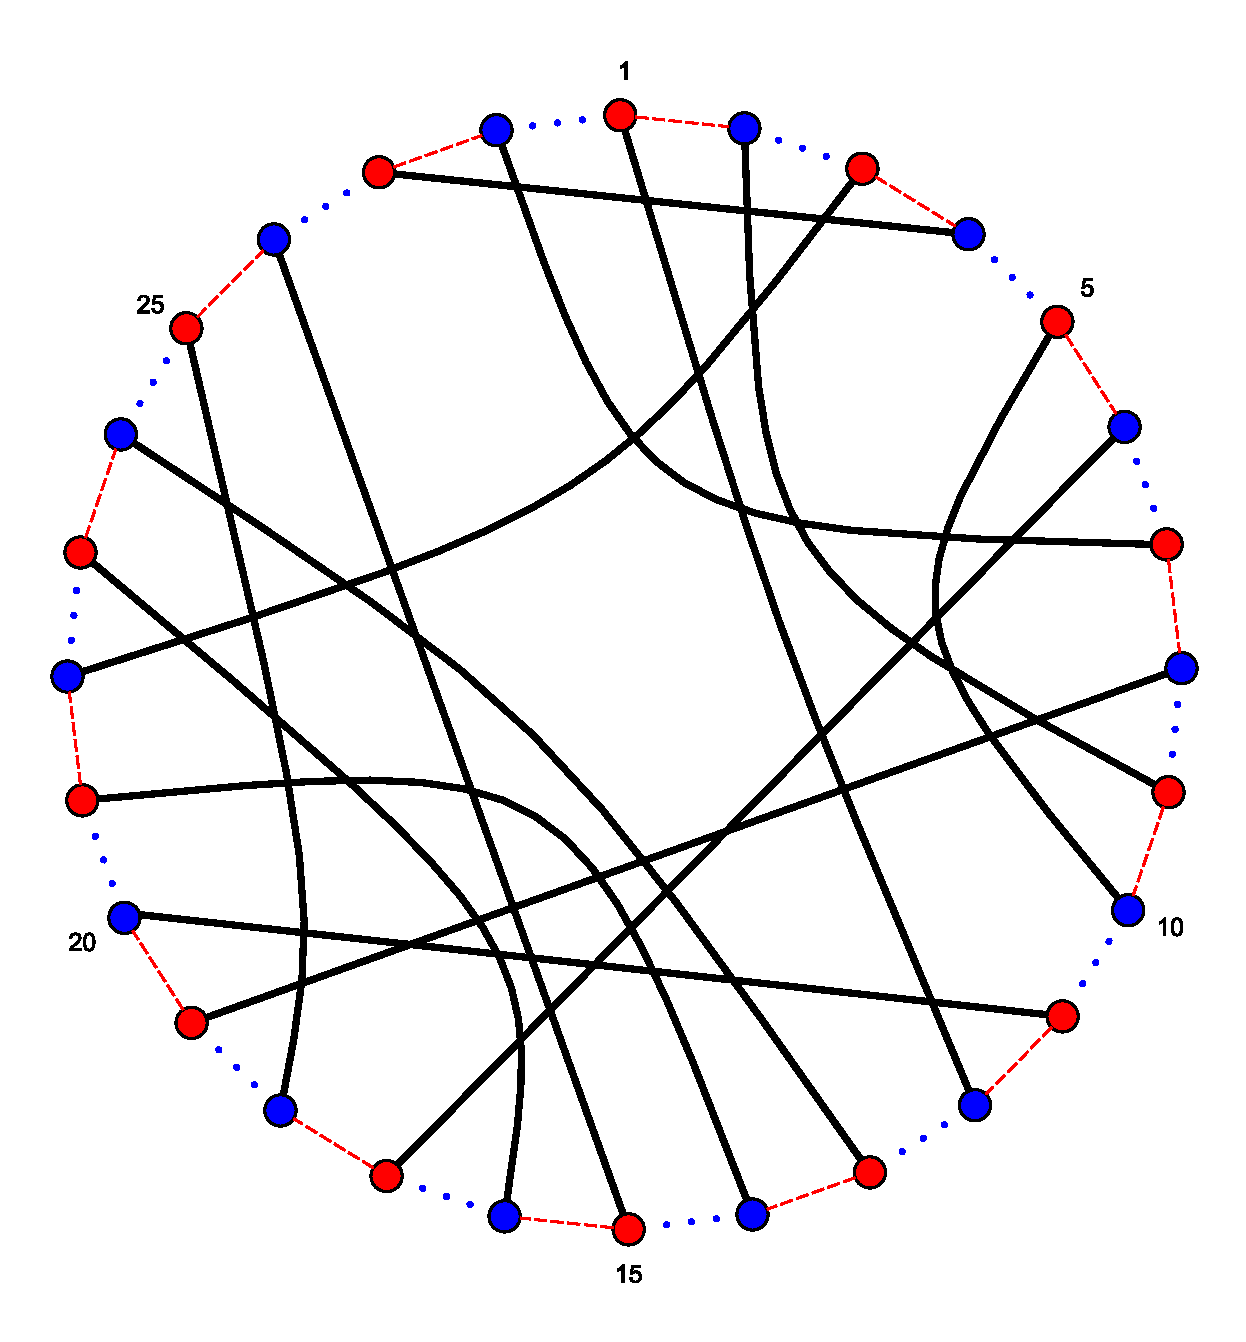
\includegraphics[width=0.5\textwidth]{../thesis/figures/two_cycles.eps}
\end{figure}
\vspace{-1em} Smallest unrestricted counterexample: $20 \leq n \leq 28$
\end{frame}

\resultFrame{4}